\documentclass[11pt]{article}
\usepackage{pgfplots}
\pgfplotsset{compat = 1.18}
\usepackage{graphicx}
\usepackage{hyperref}
\usepackage[utf8]{inputenc}
\usepackage{amsmath,amsthm,amsfonts,amssymb,amscd}
\usepackage{tikz}
\usepackage{xeCJK}
\usepackage{physics}
\usepackage{multirow,booktabs}
% \usepackage[table]{xcolor}
\usepackage{fullpage}
\usepackage{lastpage}
\usepackage{unicode-math}
\usepackage{enumitem}
\usepackage{fancyhdr}
\usepackage{mathrsfs}
\usepackage{wrapfig}
\usepackage{setspace}
\usepackage{calc}
\graphicspath{{./}}
\usepackage{multicol}
\usepackage{cancel}
\usepackage[retainorgcmds]{IEEEtrantools}
\usepackage[margin=3cm]{geometry}
\usepackage{amsmath}
\newlength{\tabcont}
\setlength{\parindent}{0.0in}
\setlength{\parskip}{0.05in}
\usepackage{empheq}
\usepackage{framed}
\usepackage[most]{tcolorbox}
\usepackage{xcolor}
\linespread{1.2}
\graphicspath{{./}}
\setCJKmainfont[AutoFakeBold = 3, AutoFakeSlant = 4]{BiauKaiTC}
\colorlet{shadecolor}{orange!15}
\parindent 0in
\parskip 12pt
\geometry{margin=1in, headsep=0.25in}
\theoremstyle{definition}
\newtheorem{thr}{Theorem}
\newtheorem{defn}{Definition}
\newtheorem{reg}{Rule}
\newtheorem{exer}{Exercise}
\newtheorem{note}{Note}
\newtheorem{asmp}{Assumption}
\begin{document}
\setcounter{section}{0}
\title{Title}

\thispagestyle{empty}
\begin{center}
  {\large \bf Programming Assignment 1 Report} \\ 
  B12901022 廖冠豪
\end{center}
\section*{Performance}
The performance of the sorting algorithms is given in the follow tables.
\subsection*{Insertion Sort}
\begin{center}
  \begin{tabular}{|c|c|c|}
    \hline 
    Input size & CPU time (s) & Memory (KB) \\ 
    \hline 
    4000.case1 & $5.552 \times 10^{-3}$ & 5904 \\ 
    \hline
    4000.case2 & $1.01 \times 10^{-4}$ & 5904 \\ 
    \hline
    4000.case3 & $8.178 \times 10^{-3}$ & 5904 \\
    \hline
    16000.case1 & $4.7489 \times 10^{-2}$ & 6056 \\ 
    \hline 
    16000.case2 & $1.02 \times 10^{-4}$ & 6056 \\ 
    \hline
    16000.case3 & $8.9745 \times 10^{-2}$ & 6056 \\ 
    \hline 
    32000.case1 & $0.180695$ & 6188 \\ 
    \hline 
    32000.case2 & $1.17 \times 10^{-4}$ & 6188 \\ 
    \hline
    32000.case3 & $0.354338$ & 6188 \\
    \hline 
    1000000.case1 & $182.187$ & 12144 \\ 
    \hline 
    1000000.case2 & $7.94 \times 10^{-4}$ & 12144 \\ 
    \hline 
    1000000.case3 & $366.832$ & 12144 \\
    \hline
  \end{tabular}
\end{center}
\subsection*{Merge Sort}
\begin{center}
  \begin{tabular}{|c|c|c|}
    \hline 
    Input size & CPU time (s) & Memory (KB) \\ 
    \hline 
    4000.case1 & $1.757 \times 10^{-3}$ & 6048 \\
    \hline
    4000.case2 & $1.446 \times 10^{-3}$ & 6048 \\
    \hline
    4000.case3 & $1.533 \times 10^{-3}$ & 6048 \\
    \hline
    16000.case1 & $5.063 \times 10^{-3}$ & 6216 \\
    \hline 
    16000.case2 & $3.519 \times 10^{-3}$ & 6216 \\
    \hline
    16000.case3 & $3.182 \times 10^{-3}$ & 6216 \\
    \hline 
    32000.case1 & $5.061 \times 10^{-3}$ & 6256 \\
    \hline 
    32000.case2 & $5.011\times10^{-3}$ & 6256 \\ 
    \hline
    32000.case3 & $6.885 \times 10^{-3}$ & 6256 \\
    \hline 
    1000000.case1 & $0.228663$ & 18288 \\ 
    \hline 
    1000000.case2 & $0.134596$ & 18288 \\ 
    \hline 
    1000000.case3 & $0.169522$ & 18288 \\
    \hline
  \end{tabular}
\end{center}
\subsection*{Bottomup Merge Sort}
\begin{center}
  \begin{tabular}{|c|c|c|}
    \hline 
    Input size & CPU time (s) & Memory (KB) \\ 
    \hline 
    4000.case1 & $2.712 \times 10^{-3}$ & 6040 \\
    \hline
    4000.case2 & $1.779 \times 10^{-3}$ & 6040 \\
    \hline
    4000.case3 & $1.613 \times 10^{-3}$ & 6040 \\
    \hline
    16000.case1 & $4.748 \times 10^{-3}$ & 6212 \\
    \hline 
    16000.case2 & $2.976 \times 10^{-3}$ & 6212 \\
    \hline
    16000.case3 & $3.343 \times 10^{-3}$ & 6212 \\
    \hline 
    32000.case1 & $7.686 \times 10^{-3}$ & 6384 \\
    \hline 
    32000.case2 & $4.384 \times 10^{-3}$ & 6384 \\
    \hline
    32000.case3 & $5.019 \times 10^{-3}$ & 6384 \\
    \hline 
    1000000.case1 & $0.215696$ & 22196 \\ 
    \hline 
    1000000.case2 & $0.125158$ & 22196 \\ 
    \hline 
    1000000.case3 & $0.136311$ & 22196 \\ 
    \hline
  \end{tabular}
\end{center}
\subsection*{Quick Sort}
\begin{center}
  \begin{tabular}{|c|c|c|}
    \hline 
    Input size & CPU time (s) & Memory (KB) \\ 
    \hline 
    4000.case1 & $8.91  \times 10^{-4}$ & 5904 \\ 
    \hline
    4000.case2 & $9.673 \times 10^{-3}$ & 5904 \\ 
    \hline
    4000.case3 & $8.564 \times 10^{-3}$ & 5904 \\ 
    \hline
    16000.case1 & $1.502  \times 10^{-3}$ & 6056 \\ 
    \hline 
    16000.case2 & $0.126353$ & 6056 \\ 
    \hline
    16000.case3 & $0.100726$ & 6428 \\ 
    \hline 
    32000.case1 & $2.879\times10^{-3}$ & 6984 \\ 
    \hline 
    32000.case2 & $0.485898$ & 6188 \\ 
    \hline
    32000.case3 & $0.354338$ & 6188 \\
    \hline 
    1000000.case1 & $8.992\times10^{-2}$ & 12144 \\ 
    \hline 
    1000000.case2 & $440.506$ & 28672 \\ 
    \hline 
    1000000.case3 & $280.635$ & 28672 \\
    \hline
  \end{tabular}
\end{center}
\subsection*{Randomized Quick Sort}
\begin{center}
  \begin{tabular}{|c|c|c|}
    \hline 
    Input size & CPU time (s) & Memory (KB) \\ 
    \hline 
    4000.case1 & $1.244 \times 10^{-2}$ & 5904 \\ 
    \hline
    4000.case2 & $1.1919 \times 10^{-2}$ & 5904 \\ 
    \hline
    4000.case3 & $1.2509 \times 10^{-2}$ & 5904 \\
    \hline
    16000.case1 & $2.26 \times 10^{-2}$ & 6056 \\ 
    \hline 
    16000.case2 & $2.5813 \times 10^{-2}$ & 6056 \\ 
    \hline
    16000.case3 & $2.5719 \times 10^{-2}$ & 6056 \\ 
    \hline 
    32000.case1 & $4.9552\times10^{-2}$ & 6188 \\ 
    \hline 
    32000.case2 & $4.6083\times 10^{-2}$ & 6188 \\ 
    \hline
    32000.case3 & $4.5859\times 10^{-2}$ & 6188 \\
    \hline 
    1000000.case1 & $1.44015$ & 12144 \\ 
    \hline 
    1000000.case2 & $1.38678$ & 12144 \\ 
    \hline 
    1000000.case3 & $1.45613$ & 12144\\
    \hline
  \end{tabular}
\end{center}
Next we plot the growth of run time as a function of the input size of the five algorithms in the following charts. Each chart stands for the run time for one test case(average case, worst case, best case). After plotting the run time of the algorithms on log scale, we then calculate the slope of the trendline by linear regression(i.e. finding the line on the 2D plane with the smallest sum of square of distance to each point.) \\ 
\subsection*{Average Case}
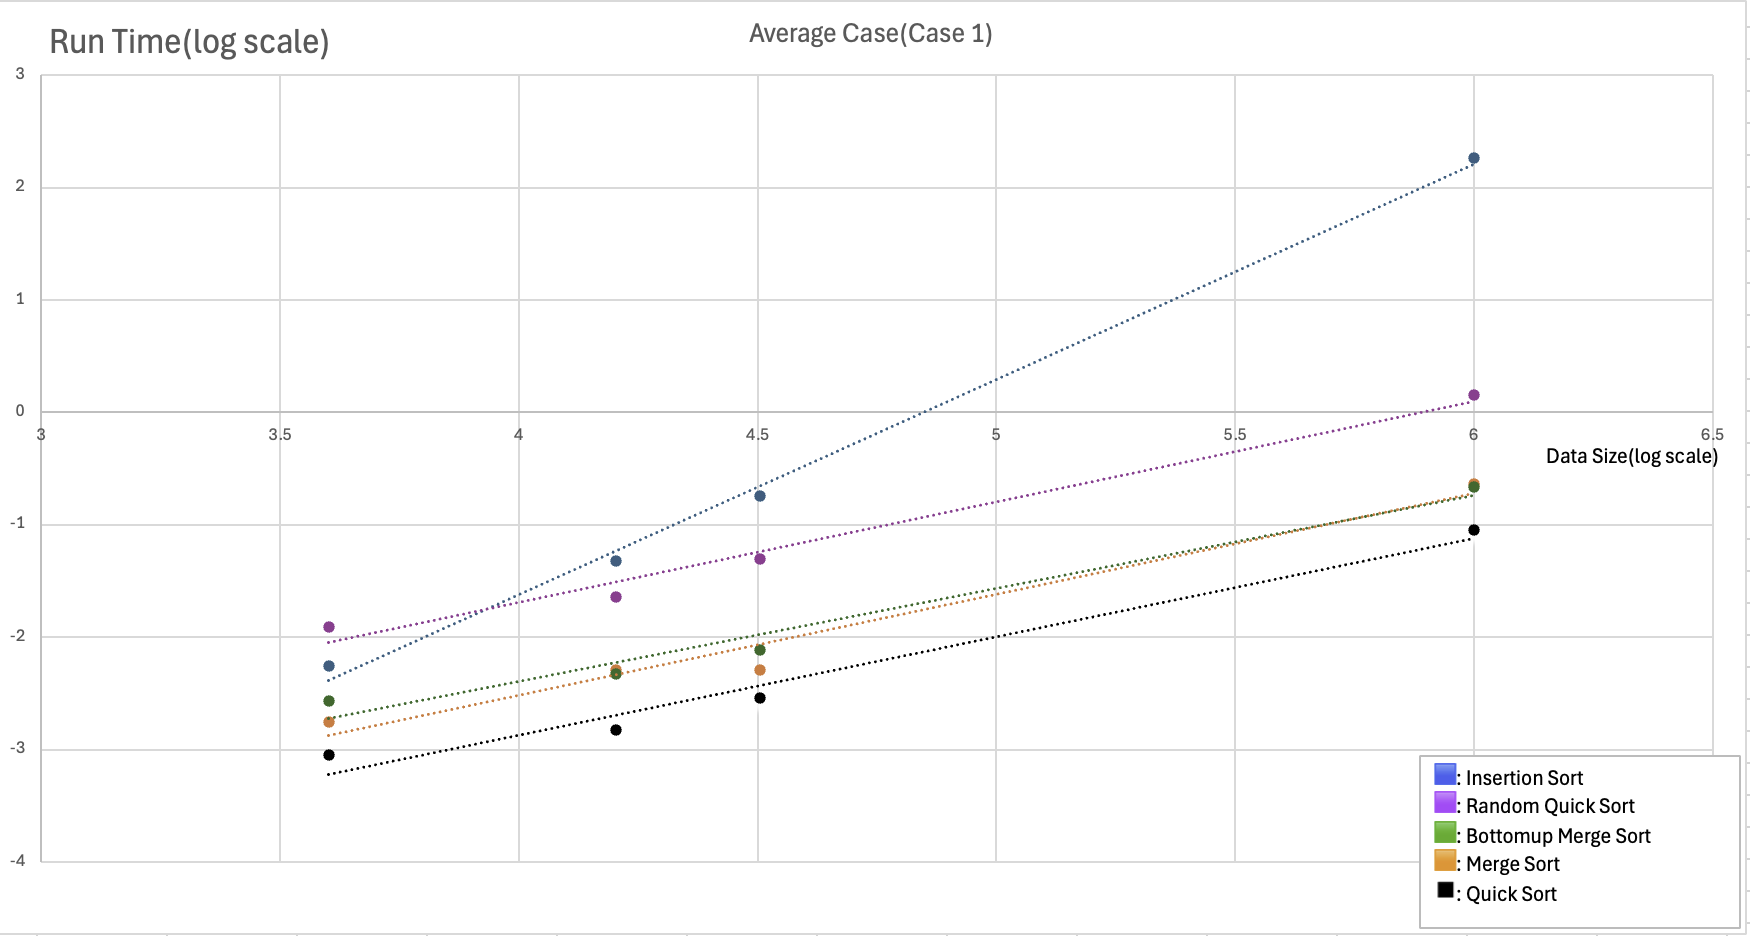
\includegraphics[width = \textwidth]{Chart 1.png}
\subsubsection*{slope}
\begin{itemize}
  \item IS: 1.9118
  \item RQS: 0.9018
  \item MS: 0.8968 
  \item BMS: 0.8267
  \item QS: 0.8745
\end{itemize}
\subsection*{Best Case}
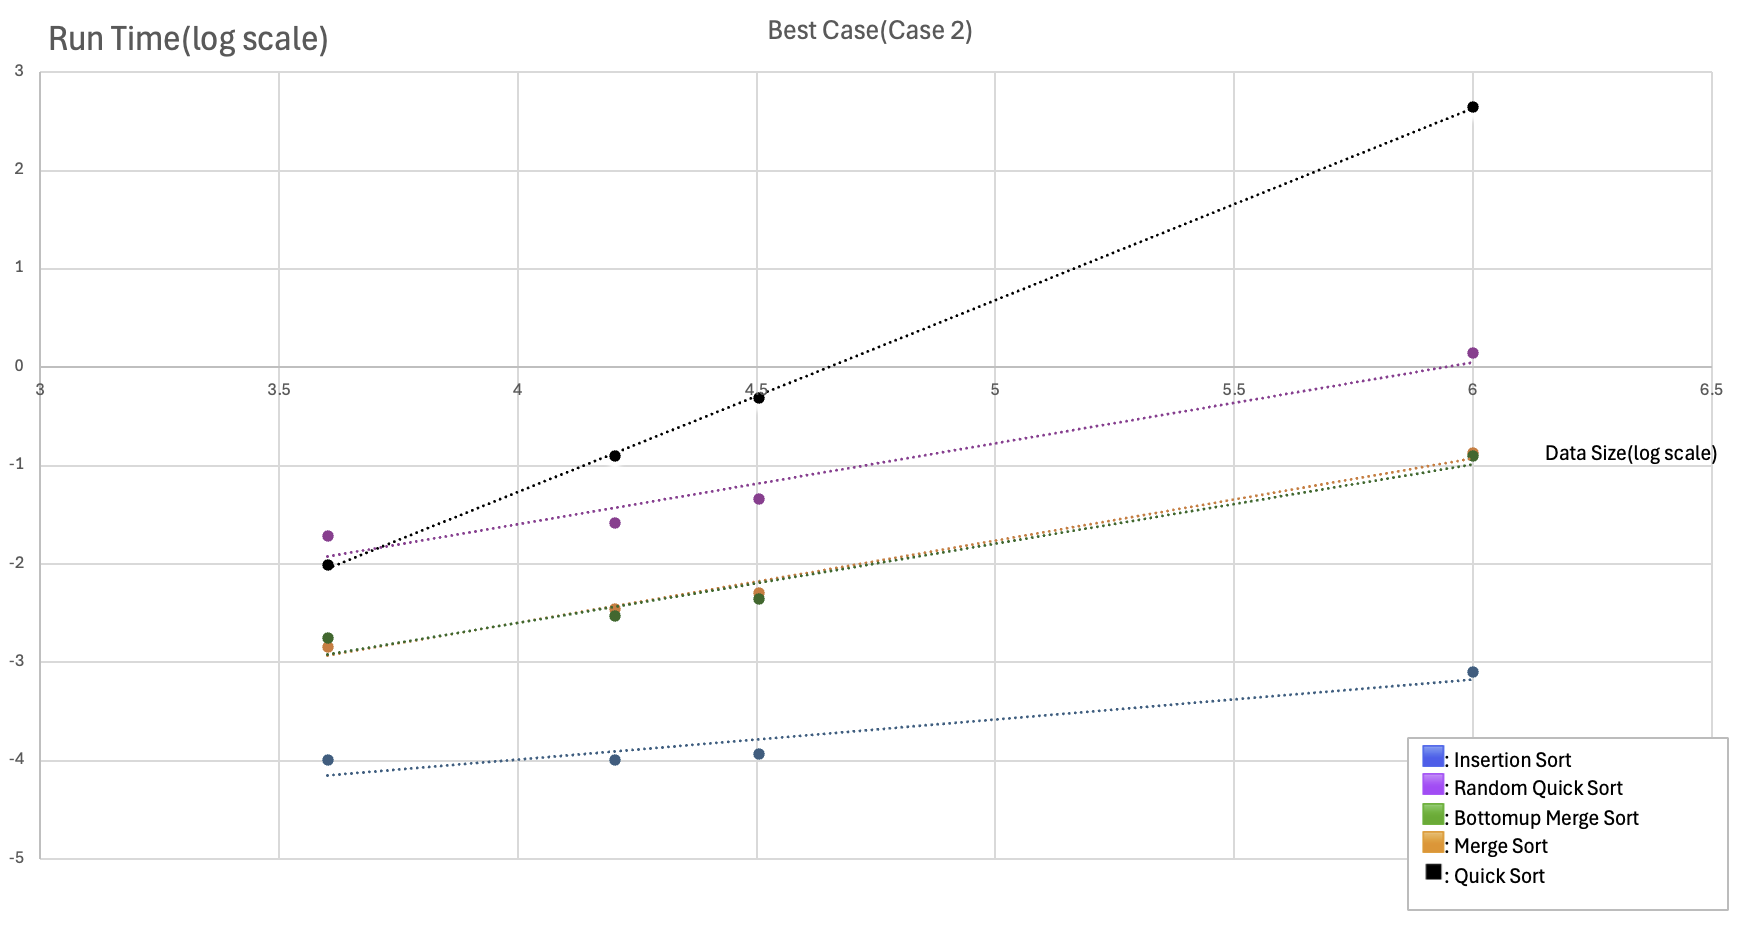
\includegraphics[width = \textwidth]{Chart 2.png}
\subsubsection*{slope}
\begin{itemize}
  \item IS: 0.4062
  \item RQS: 0.8232
  \item MS: 0.8387 
  \item BMS: 0.8062
  \item QS: 1.9503
\end{itemize}
\subsection*{Worst Case}
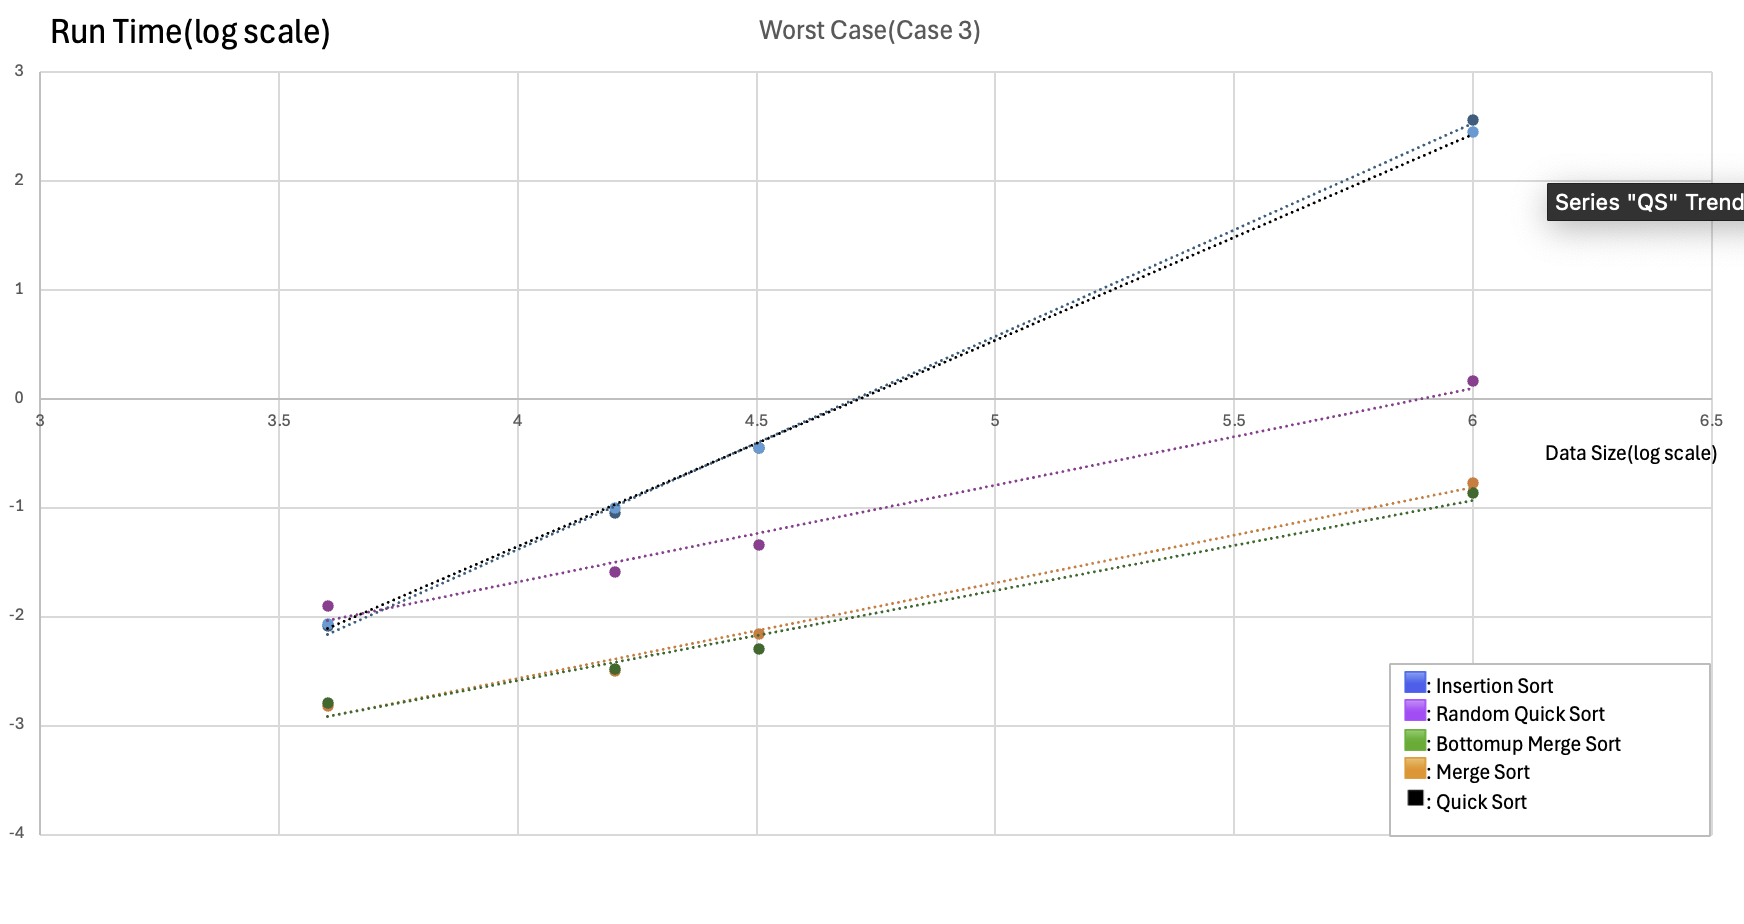
\includegraphics[width = \textwidth]{Chart 3.png}
\begin{itemize}
  \item IS: 1.9579
  \item RQS: 0.8912
  \item MS: 0.8785 
  \item BMS: 0.8290
  \item QS: 1.8912
\end{itemize}
\newpage
\section*{Discussion}
% We see that for insertion sort, the slope is approximately $2$ in average and worst case, and is approximately $1$ in best case. This fits the complexity in the text book, as the complexity for insertion sort is $\Theta(n^2)$ in average ans worst case, and $\Theta(n)$ in best case. For merge sort and bottomup merge sort the slope is approximately $1$, this also fits the complexity in the text book, as the complexity for merge sort and buttomup merge sort in all cases is $\Theta(n\lg{n})$, and the effect of the $\lg{n}$ is insignificant on log scale. For quick sort, the slope is approximately $1$ in the average case, and is approximately $2$ in the worst and best cases. This also fits the complexity in the text book, as the complexity for quick sort is $n\lg{n}$ for the average case, and the complexity is $\Theta(n^2)$ when the array is already sorted(worst and best case). The slope for randomized quick sort is also approximately $1$ for all the three cases, as the $\Theta(n^2)$ worst case is unlikely to happen when the pivot is randomly chosen. \\ 
% Furthermore, we see that compared with other $\Theta(n\lg{n})$ algorithms, randomized quick sort can be slower, this may be because that in the process of randomly choosing the pivot position, modular operation is conducted and the a pseudorandom number is generated, these operations is more expensive(time-costing) than the operations used in merge sort and bottomup merge sort(e.g. addition, access of array elements...), so the runtime of randomized quick sort is larger than that of merge sort and bottomup merge sort by a constant factor(the complexity remains the same and hence the slope on log scale). \\ 
We compare the slope of each algorithm in every case to the complexity provided in the textbook. 
\subsubsection*{Insertion Sort}
The complexity provided in the textbook for IS is $\Theta(n^2)$ for average and worst case and $\Theta(n)$ for best case. \\ 
For average and worst case, the slope of its run time to input size on log scale is only slightly less than the theoretical value $2$. This deviation may be due to the effect of terms lower than $n^2$ in IS's runtime. When analyzing the run time, only asymptotic behaviour is of interest and the lower terms are neglected. But in practice, the lower terms still plays a role in the total run time and slightly lower the slope at which the run time grows. \\ 
For the best case, the slope differs significantly from the theoretical value $1$. This may be because that for the given input size and the power of c++/c, the time needed to finish the $\Theta(n)$ operation(n times of accessing elements of the array and comparing between integers), is too little(i.e. small constant for the $\Theta(n)$ term), so the slope is greatly affected by other processes in the algorithm or CPU with lower complexity but larger constants.
\subsubsection*{Merge Sort, Buttomup Merge sort, Randomized Quick Sort}
The complexity in the textbook for the three algorithms is $\Theta(n\lg{n})$ for all cases. (For RQS the case where it becomes $\Theta(n^2)$ still exists, but is extremely unlikely if the pivot is randomly chosen) \\
We see that the slop of these algorithms in the three cases range between $0.80$ and $0.90$, which is slightly smaller than the theoretical value $1$(the $\lg{n}$ term can be neglected on log scale asymptotically). The reason for this deviation is similar to the case in IS. For the input size for the assignment, the difference between the leading $\Theta(n\lg{n})$ term and other terms(e.g. $\Theta(n)$ terms) isn't large enough for the effect of the lower terms to be complete neglected. Therefore the slope obtained here is slightly smaller than the theoretical value which the algorithms should show asymptotically.
\subsubsection*{Quick Sort}
The complexity in the textbook for QS is $\Theta(n\lg{n})$ for average case and $\Theta(n^2)$ for the best and worst case(in both the array is already sorted). \\ 
The slope in the best and worst cases is similar to the slope of IS in the average and worst case, where both algorithms run under $\Theta(n^2)$ complexity. For the average case the slope is similar to that of MS, BMS and RQS, where the algorithms all run under $\Theta(n\lg{n})$ complexity. The slope in each case is also slightly less than the corresponding theoretical value, for reasons discussed above.
\section*{Comparison}
\subsection*{MS vs. BMS}
We see that the runtime of MS and BMS are really close, but BMS is faster by a slight margin. This is because no recursive function calls is made in BMS, which could save some time. Also, in all three cases the slope of MS is larger than BMS, that is, closer to the theoretical value. This may be due to the fact that since the $\Theta(n\lg{n})$ part of MS is slower than that of BMS, the effect of the leading term on the slope is less affected by the lower terms.
\subsection*{QS vs. RQS}
In case 1 and case 3, RQS runs a lot faster than QS, as the complexity for RQS is $\Theta(n\lg{n})$ while that for QS is $\Theta(n^2)$. However, wee see that in case 2, when both the algorithms run at $\Theta(n\lg{n})$ complexity, quick sort is faster than randomized quick sort. This is because the process of randomly selecting the pivot position involves generating a random number and modular operation, which is more time-consuming than other $\Theta(1)$ operations used in quick sort and the constant for QS is larger than that of RQS when both run under $\Theta(n\lg{n})$ complexity. \\ 
When encountered with a already sorted array, QS performs like IS, with $\Theta(n^2)$ complexity, which can is inefficient. By the comparison between QS and RQS we see that this problem is effectively solved by choosing the pivot position randomly every time when partitioning the array, that is, choosing RQS over QS.
\section*{Data Structures}
\begin{itemize}
  \item std::vector
\end{itemize}
\newpage
\section*{Other Findings}
By comparison between the five algorithms, I've noticed that the difference between the calculated slope and the theoretical(asymptotic) slope for each algorithm is negative related to the rate at which the leading term of the algorithm. As demonstrated below
\begin{gather*}
  \Theta(n^2)(\text{IS(average \& worst case), QS(best \& worst case)}) \approx 5\%  \\
  < \Theta(n\lg{n})(\text{MS, BMS, RQS, QS(average case)}) \approx 15\% \\ 
  < \Theta(n)(\text{IS(best case)}) \approx 50\%
\end{gather*}
The percentage is given by dividing the difference between the actual slope and the theoretical slope and dividing it by the theoretical slope. This is because the slower the leading term grows, the smaller the difference between it and the lower terms is, and hence the effect of the lower terms is more significant. \\ 
(This is just my guess, but I find it interesting and convincing at least to myself)



\end{document}

